% Theory §4B: Gradient Conflict Proposition
% To be integrated into the ICLR 2027 paper §3.2

\subsection{Gradient Conflict in Joint Training}
\label{sec:gradient-conflict}

We complement the capacity bound with an optimisation-level observation:
even when capacity is sufficient, joint training can induce conflicting
gradient signals on the shared encoder.

\begin{proposition}[Gradient conflict]
\label{prop:gradient-conflict}
Let $\theta_{\mathrm{enc}}$ denote the shared encoder parameters in a
coupled autoencoder trained with loss
$\mathcal{L} = (1{-}\varphi)\,\mathcal{L}_{\mathrm{rec}} +
\varphi\,\mathcal{L}_{\mathrm{fcst}}$.
Let $\mathbf{g}_r = \nabla_{\theta_{\mathrm{enc}}} \mathcal{L}_{\mathrm{rec}}$
and $\mathbf{g}_f = \nabla_{\theta_{\mathrm{enc}}} \mathcal{L}_{\mathrm{fcst}}$.
If $\langle \mathbf{g}_r, \mathbf{g}_f \rangle < 0$
(i.e.\ their cosine similarity is negative), then for any
$\varphi \in (0,1)$ the combined gradient
$\mathbf{g}_\varphi = (1{-}\varphi)\,\mathbf{g}_r + \varphi\,\mathbf{g}_f$
satisfies:
\begin{enumerate}
\item[\emph{(a)}] \textbf{Suboptimality:}
  $\langle \mathbf{g}_\varphi, \mathbf{g}_r \rangle < \lVert \mathbf{g}_r \rVert^2$
  and
  $\langle \mathbf{g}_\varphi, \mathbf{g}_f \rangle < \lVert \mathbf{g}_f \rVert^2$.
  A step along $-\mathbf{g}_\varphi$ decreases each objective strictly less
  than the corresponding individual gradient direction.
\item[\emph{(b)}] \textbf{Cancellation:}
  $\lVert \mathbf{g}_\varphi \rVert^2
  < (1{-}\varphi)^2 \lVert \mathbf{g}_r \rVert^2
  + \varphi^2 \lVert \mathbf{g}_f \rVert^2$.
  Gradient magnitude is reduced by inter-task cancellation;
  the deficit $2\varphi(1{-}\varphi)\lvert\langle\mathbf{g}_r,\mathbf{g}_f\rangle\rvert$
  quantifies the wasted optimisation effort.
\item[\emph{(c)}] \textbf{Extreme weighting:}
  There exist thresholds $0 < \varphi_{\mathrm{lo}} < \varphi_{\mathrm{hi}} < 1$
  such that for $\varphi > \varphi_{\mathrm{hi}}$ the update $-\mathbf{g}_\varphi$
  actively increases $\mathcal{L}_{\mathrm{rec}}$, and for
  $\varphi < \varphi_{\mathrm{lo}}$ it actively increases
  $\mathcal{L}_{\mathrm{fcst}}$.
\end{enumerate}
In the decoupled architecture, the forecasting pathway has no dependence on
$\theta_{\mathrm{enc}}$, so
$\mathbf{g}_f = \mathbf{0}$ and no conflict arises.
\end{proposition}

\begin{proof}
Expanding the inner products:
\begin{align}
  \langle \mathbf{g}_\varphi, \mathbf{g}_r \rangle
  &= (1{-}\varphi)\lVert \mathbf{g}_r \rVert^2
     + \varphi\,\langle \mathbf{g}_f, \mathbf{g}_r \rangle, \label{eq:ip-r}\\
  \langle \mathbf{g}_\varphi, \mathbf{g}_f \rangle
  &= (1{-}\varphi)\langle \mathbf{g}_r, \mathbf{g}_f \rangle
     + \varphi\,\lVert \mathbf{g}_f \rVert^2. \label{eq:ip-f}
\end{align}

\emph{Part (a).}
Since $\varphi > 0$ and $\langle \mathbf{g}_f, \mathbf{g}_r \rangle < 0$,
the second term of~\eqref{eq:ip-r} is strictly negative, giving
$\langle \mathbf{g}_\varphi, \mathbf{g}_r \rangle
< (1{-}\varphi)\lVert \mathbf{g}_r \rVert^2 + \varphi\lVert \mathbf{g}_r \rVert^2
= \lVert \mathbf{g}_r \rVert^2$.
The argument for $\mathbf{g}_f$ via~\eqref{eq:ip-f} is symmetric.

\emph{Part (b).}
$\lVert \mathbf{g}_\varphi \rVert^2
= (1{-}\varphi)^2\lVert\mathbf{g}_r\rVert^2
+ 2\varphi(1{-}\varphi)\langle\mathbf{g}_r,\mathbf{g}_f\rangle
+ \varphi^2\lVert\mathbf{g}_f\rVert^2$.
The cross-term is strictly negative.

\emph{Part (c).}
From~\eqref{eq:ip-r},
$\langle \mathbf{g}_\varphi, \mathbf{g}_r \rangle < 0$
iff $\varphi > \lVert\mathbf{g}_r\rVert^2
/ (\lVert\mathbf{g}_r\rVert^2 + \lvert\langle\mathbf{g}_f,\mathbf{g}_r\rangle\rvert)$.
Set $\varphi_{\mathrm{hi}}$ to this value; it lies in $(0,1)$.
Symmetrically, $\langle\mathbf{g}_\varphi,\mathbf{g}_f\rangle < 0$
iff $\varphi < \varphi_{\mathrm{lo}}
= \lvert\langle\mathbf{g}_r,\mathbf{g}_f\rangle\rvert
/ (\lVert\mathbf{g}_f\rVert^2 + \lvert\langle\mathbf{g}_r,\mathbf{g}_f\rangle\rvert)$.
By Cauchy--Schwarz,
$\lvert\langle\mathbf{g}_r,\mathbf{g}_f\rangle\rvert
< \lVert\mathbf{g}_r\rVert\lVert\mathbf{g}_f\rVert$
(strict when $\mathbf{g}_r \not\parallel \mathbf{g}_f$), which gives
$\varphi_{\mathrm{lo}} < \varphi_{\mathrm{hi}}$.
\end{proof}

\paragraph{Empirical verification.}
We train coupled Koopman autoencoders at $\varphi \in \{0.05, 0.1, 0.25,
0.5, 0.75, 0.9\}$ and log $\cos(\mathbf{g}_r, \mathbf{g}_f)$ at the
encoder parameters every 10 batches. Figure~\ref{fig:gradient-conflict}
shows that \textbf{the cosine similarity is negative 62--92\% of the time}
across all systems and $\varphi$ values, with mean cosine ranging from
$-0.233$ to $-0.032$. The conflict persists throughout training and does
not resolve as optimisation progresses.

This connects to the multi-task optimisation literature: PCGrad
\citep{yu2020gradient} and CAGrad \citep{liu2021conflict} mitigate gradient
conflict by projecting or rescaling conflicting gradients.  Our decoupling
approach takes a different route: it removes the shared parameters that
give rise to the conflict.

\begin{figure}[t]
\centering
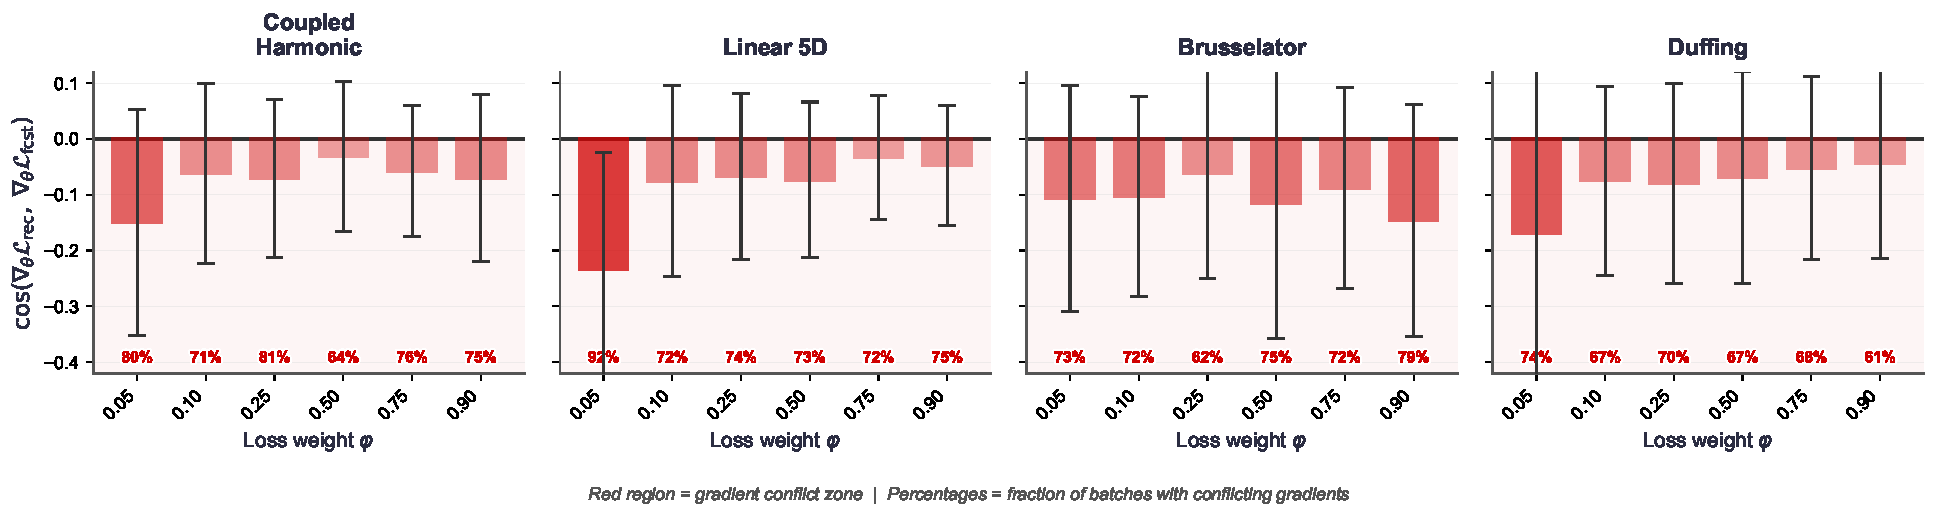
\includegraphics[width=\textwidth]{gradient_conflict.png}
\caption{Cosine similarity between reconstruction and forecasting
gradients at the shared encoder during coupled training.  Red bars
indicate negative mean cosine (gradient conflict).  Percentages show
the fraction of training batches with negative cosine.  The conflict
is persistent across all $\varphi$ values and all systems.}
\label{fig:gradient-conflict}
\end{figure}
